% Dialect sketch and future golden input. Invented content only — this deck
% is about leantex itself; nothing here derives from any private document.
% Preamble syntax is NOT final. M5 target: slides — frames, overlays, speaker
% notes, verbatim code with font fallbacks, external figures, and the
% external-render escape hatch.

\documentclass[aspectratio=169]{slides}

\fonts{
  body = "IBM Plex Sans",
  mono = "IBM Plex Mono",
}
% Code samples mix scripts and symbols; fall back per glyph.
\fontfallback{ mono <- "DejaVu Sans Mono" }

\pdfmeta{ title = "leantex: a dummy deck" }

\begin{document}

\begin{frame}{Layout is a value}
  \begin{itemize}
    \item<1-> Assertions fail builds, not readers.
    \item<2-> Metrics are queryable, not measured by hand.
    \item<3-> Heavy machinery stays behind boundaries until absorbed.
  \end{itemize}
  \note{Speaker notes render only in the second-screen notes build.}
\end{frame}

\begin{frame}{Porcelain}
  \begin{verbatim}
$ leantex build deck.tex
assert pages == 12 ......... ok
external tikz .............. 2 boxes (cache hit)
fallback glyphs: λ ⊗ ∑ ≈ ↦
  \end{verbatim}
\end{frame}

\begin{frame}{Figures}
  % External asset placed as a measured box: PDF page (vector), PNG, or JPEG.
  \figure[width = 0.6\textwidth]{figures/diagram.pdf}
\end{frame}

\begin{frame}{Escape hatch}
  % Handed to a declared, pinned external renderer, cached by content hash,
  % placed as an opaque measured box.
  \begin{external}[tikz]
    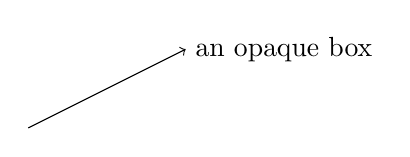
\begin{tikzpicture}
      \draw[->] (0,0) -- (2,1) node[right] {an opaque box};
    \end{tikzpicture}
  \end{external}
\end{frame}

\end{document}
